\begin{frame}{Two-Set Venn Diagram}
\begin{center}
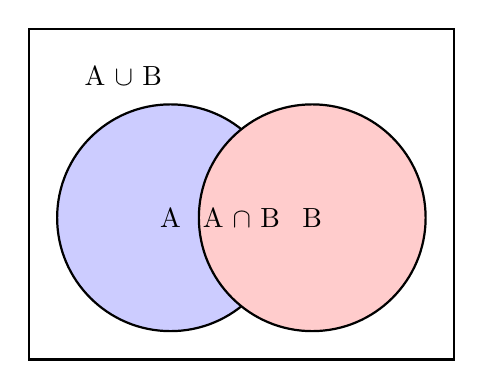
\begin{tikzpicture}[scale=1.2]
    \draw[thick, fill=blue!20] (0,0) circle (1.2);
    \draw[thick, fill=red!20] (1.5,0) circle (1.2);
    \draw[thick] (-1.5,-1.5) rectangle (3,2);
    
    \node at (0,0) {A};
    \node at (1.5,0) {B};
    \node at (0.75,0) {A $\cap$ B};
    \node at (-0.5,1.5) {A $\cup$ B};
\end{tikzpicture}
\end{center}

\footnotesize
\texttt{\textbackslash draw[thick, fill=blue!20] (0,0) circle (1.2);}\\
\texttt{\textbackslash draw[thick, fill=red!20] (1.5,0) circle (1.2);}
\end{frame}